
\begin{titlepage}
	
	\newcommand{\HRule}{\rule{\linewidth}{0.5mm}} % Defines a new command for the horizontal lines, change thickness here
	
	\center % Center everything on the page
	
	%----------------------------------------------------------------------------------------
	%	HEADING SECTIONS
	%----------------------------------------------------------------------------------------
	
\textsc{\LARGE Bridging the Gap Engineering}\\[0.5cm] % Name of your university/college
\textsc{\Large Pre-Qualified Bridge Proposal}\\[0.5cm] % Major heading such as course name
\textsc{\large Begley Road, Cabell County, WV}\\[0.5cm]
%	TITLE SECTION
%----------------------------------------------------------------------------------------

\HRule \\[0.4cm]
 \huge \bfseries Final Report\\[0.1cm] % Title of your document
\HRule \\[1.5cm]

%----------------------------------------------------------------------------------------
%	AUTHOR SECTION
%----------------------------------------------------------------------------------------

\begin{minipage}{1.0\textwidth}
	\begin{flushleft} \large
		
		\emph{Contributors:}\\  %italicizes contributors, there are other commands for this but they are less "safe" so they aren't recommended
		Brandon \textsc{Adams},
		Michael \textsc{Ashworth},
		Zachary \textsc{Cumm},
		Brandon \textsc{Dial},		
		\begin{center}
			Natasha \textsc{Napier},
			John \textsc{Skaggs}			
		\end{center}
	\end{flushleft}
\end{minipage}
~
%\begin{minipage}{0.4\textwidth}
%\begin{flushright} \large
%\emph{Professor:} \\
%Dr. Isaac \textsc{Wait} % Supervisor's Name
%\end{flushright}
%\end{minipage}\\[2cm]

% If you don't want a supervisor, uncomment the two lines below and remove the section above
%\Large \emph{Author:}\\
%John \textsc{Smith}\\[3cm] % Your name

%----------------------------------------------------------------------------------------
%	DATE SECTION
%----------------------------------------------------------------------------------------
%{\large \today}\\[2cm] % Date, change the \today to a set date if you want to be precise

%----------------------------------------------------------------------------------------
%	LOGO SECTION
%----------------------------------------------------------------------------------------
\vspace{2.0cm} %change positioning of logo

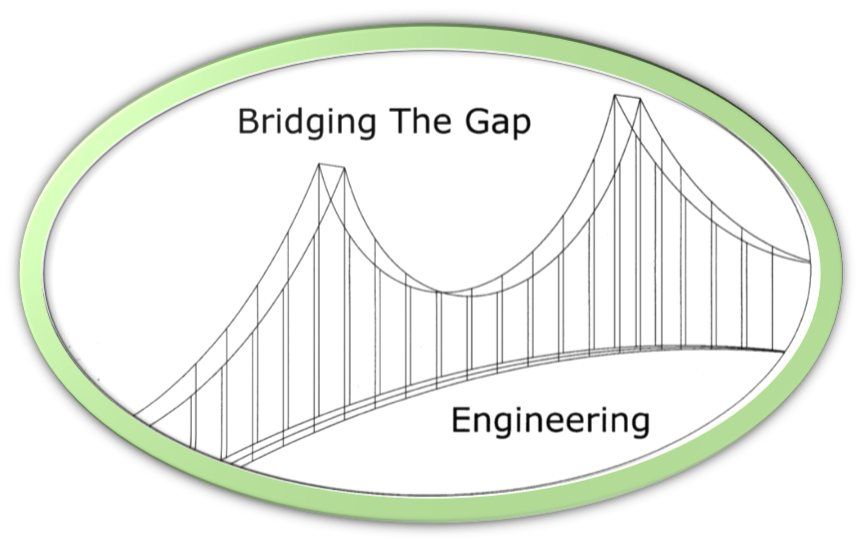
\includegraphics[width=0.75\linewidth, scale=1.5]{appendix/logoo}
\label{fig:logoo}



%----------------------------------------------------------------------------------------

\vfill % Fill the rest of the page with whitespace

\end{titlepage}

\newpage